\section{fusion\_\-random\_\-t Class Reference}
\label{classfusion__random__t}\index{fusion\_\-random\_\-t@{fusion\_\-random\_\-t}}
Inheritance diagram for fusion\_\-random\_\-t:\nopagebreak
\begin{figure}[H]
\begin{center}
\leavevmode
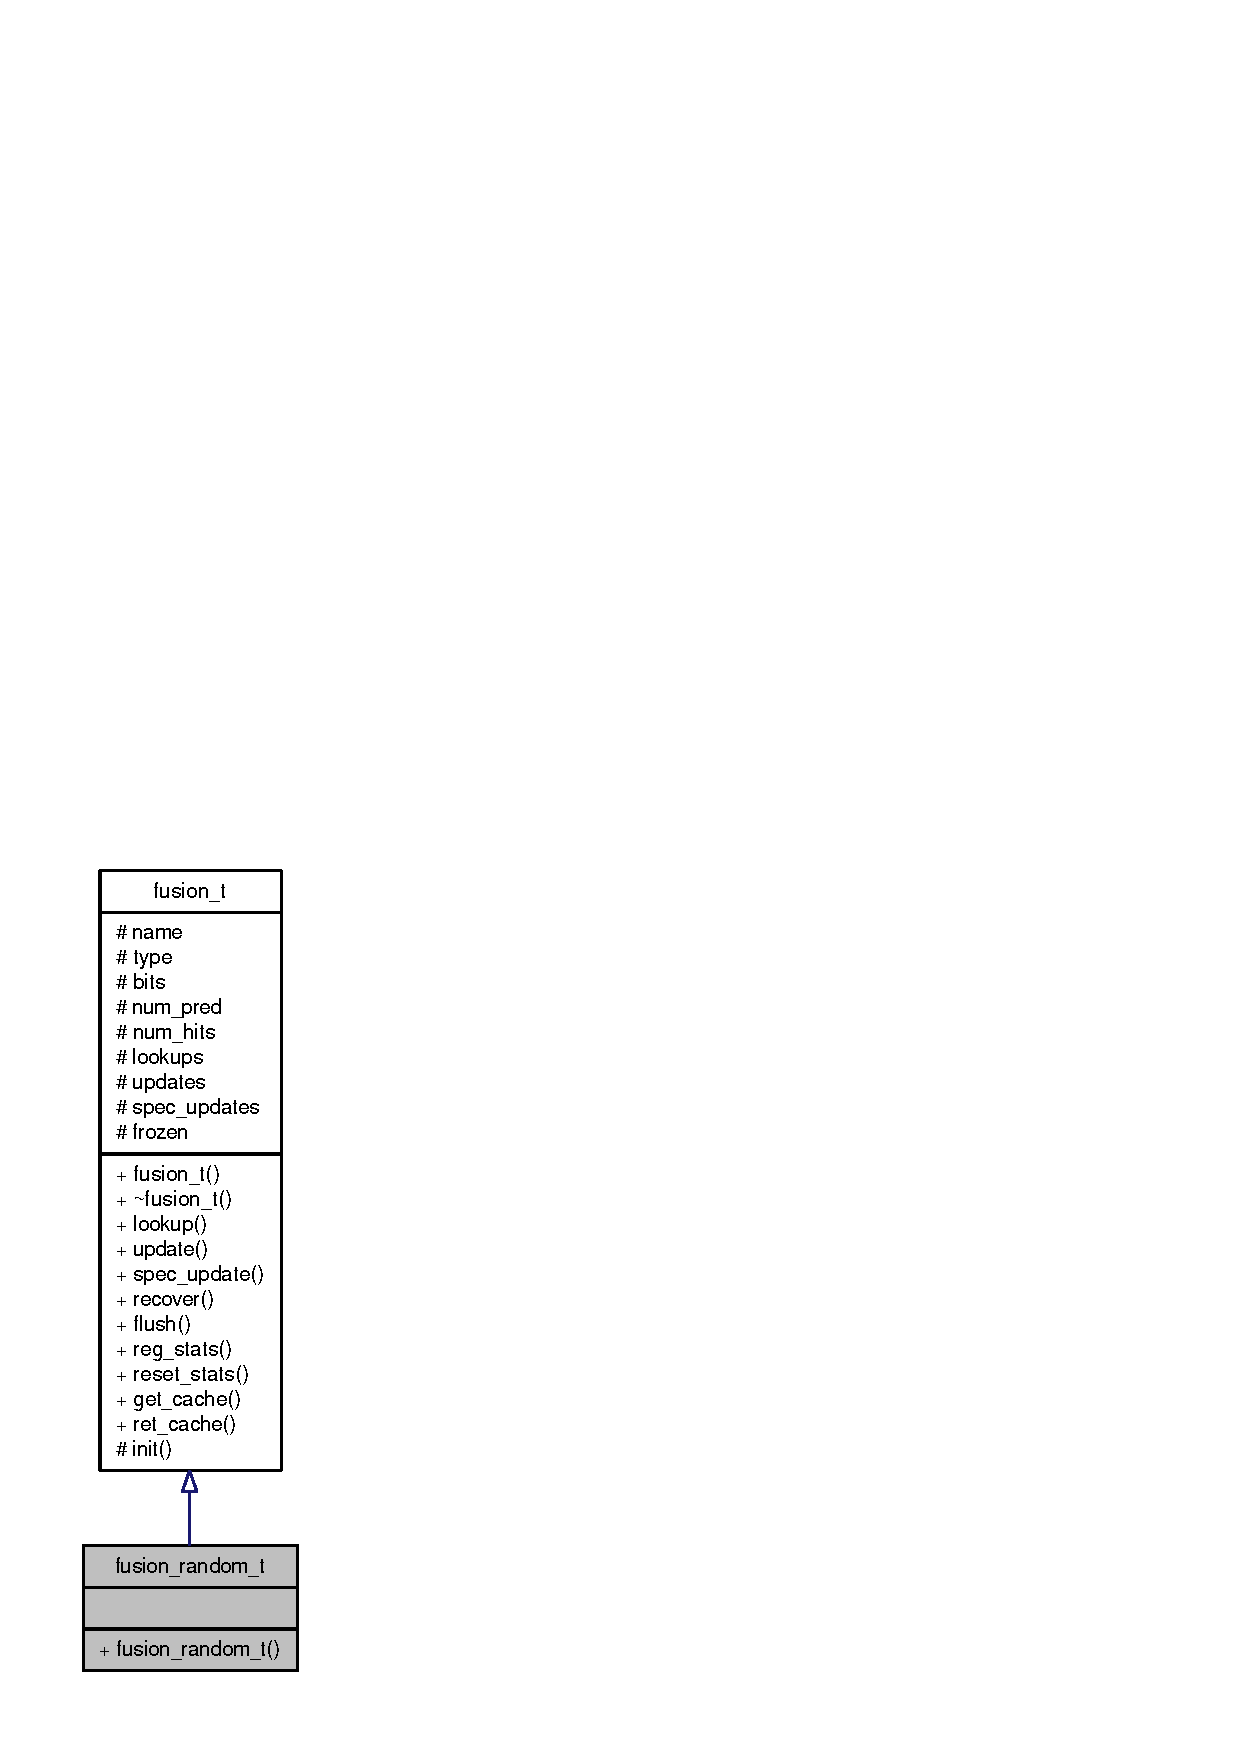
\includegraphics[height=400pt]{classfusion__random__t__inherit__graph}
\end{center}
\end{figure}
Collaboration diagram for fusion\_\-random\_\-t:\nopagebreak
\begin{figure}[H]
\begin{center}
\leavevmode
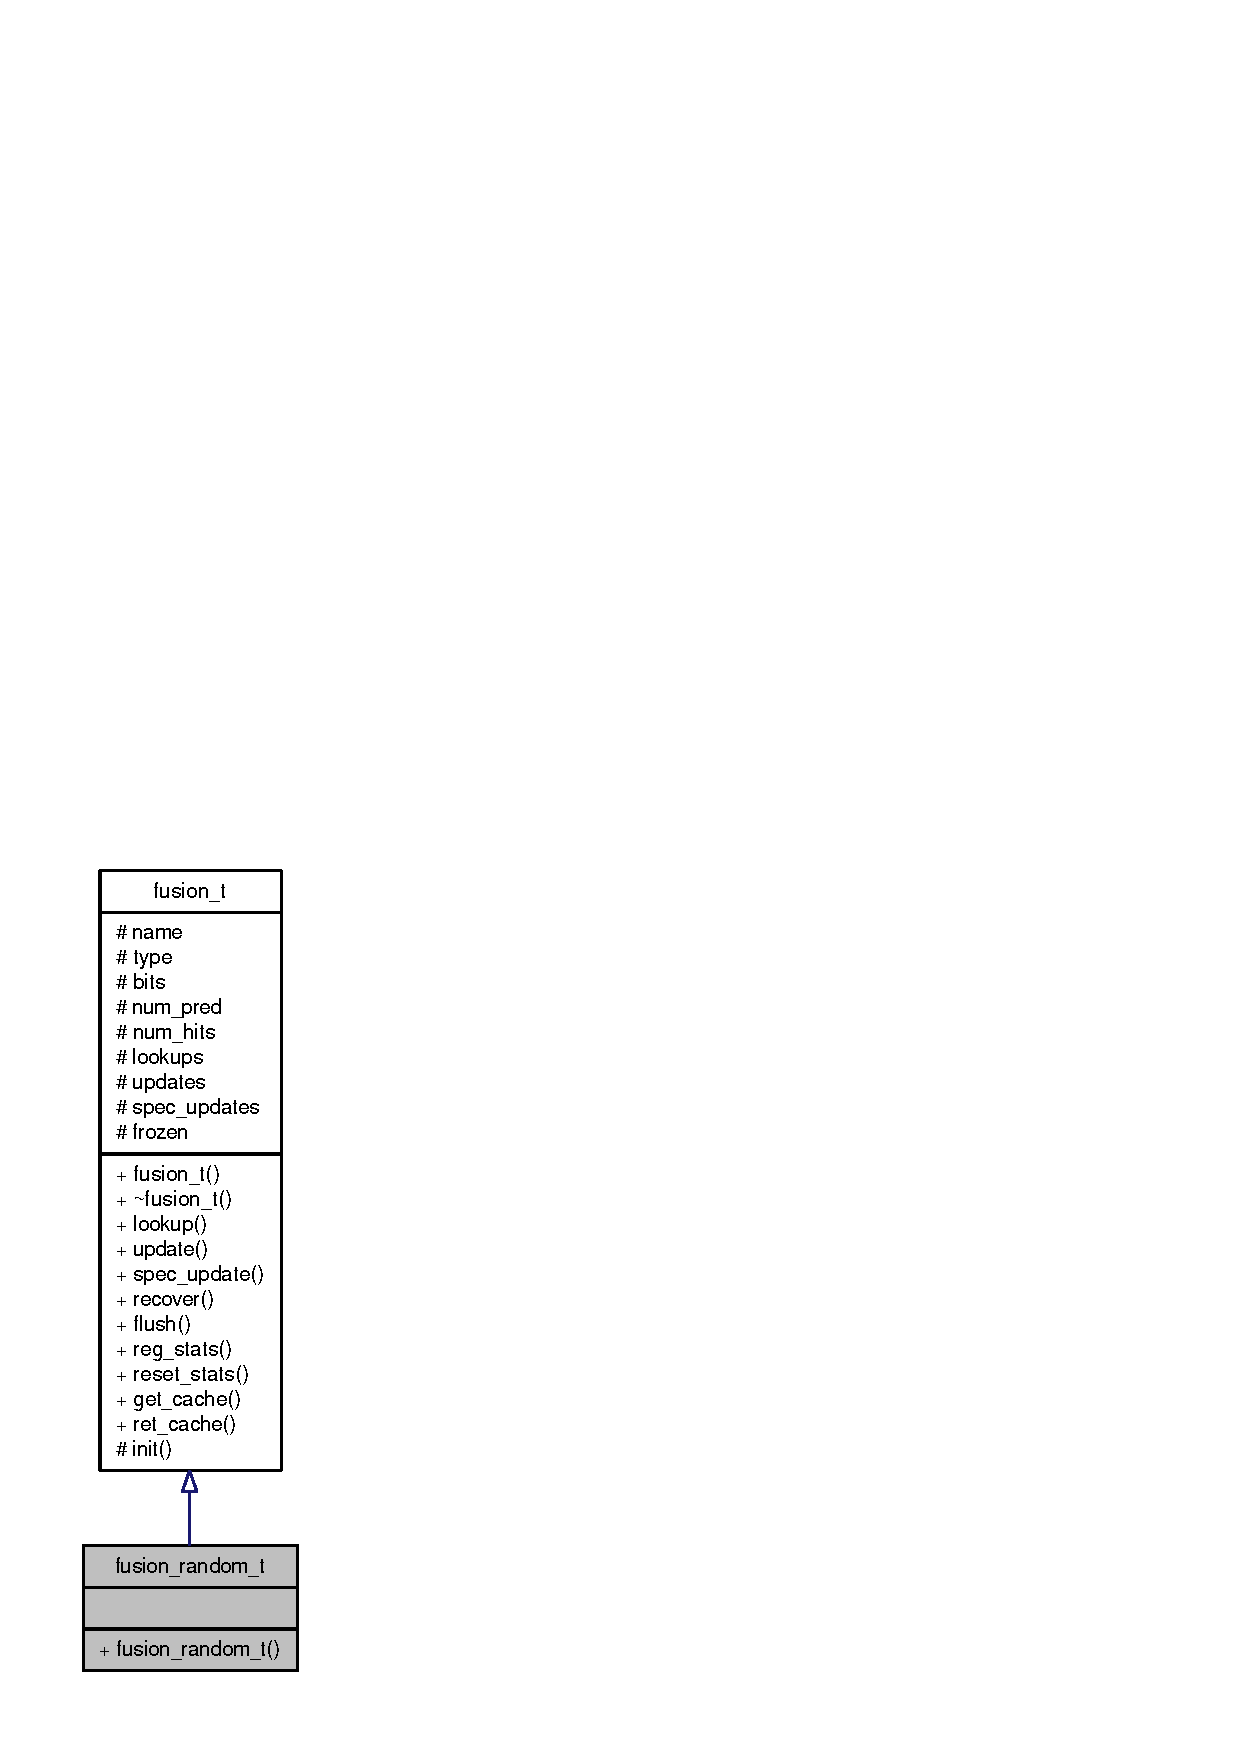
\includegraphics[height=400pt]{classfusion__random__t__coll__graph}
\end{center}
\end{figure}
\subsection*{Public Member Functions}
\begin{CompactItemize}
\item 
{\bf fusion\_\-random\_\-t} (const int arg\_\-num\_\-pred)
\end{CompactItemize}


\subsection{Detailed Description}


Definition at line 15 of file fusion-random.cpp.

\subsection{Constructor \& Destructor Documentation}
\index{fusion\_\-random\_\-t@{fusion\_\-random\_\-t}!fusion\_\-random\_\-t@{fusion\_\-random\_\-t}}
\index{fusion\_\-random\_\-t@{fusion\_\-random\_\-t}!fusion_random_t@{fusion\_\-random\_\-t}}
\subsubsection[{fusion\_\-random\_\-t}]{\setlength{\rightskip}{0pt plus 5cm}fusion\_\-random\_\-t::fusion\_\-random\_\-t (const int {\em arg\_\-num\_\-pred})\hspace{0.3cm}{\tt  [inline]}}\label{classfusion__random__t_c7a64dc43d150d5995100b3e6a6a92ca}




Definition at line 20 of file fusion-random.cpp.

References fusion\_\-t::bits, COMPONENT\_\-NAME, fatal(), fusion\_\-t::init(), fusion\_\-t::name, fusion\_\-t::num\_\-pred, and fusion\_\-t::type.

The documentation for this class was generated from the following file:\begin{CompactItemize}
\item 
{\bf fusion-random.cpp}\end{CompactItemize}
